%%
%% Beuth Hochschule für Technik 
%%
%% Einleitung 1
%%
%%

\newpage
[Hansert]
\section{Zu regelndes Objekt kennen lernen}
Das Objekt was wir regeln sollen handelt sich um einen elektrischen steuerbaren hydraulischen Druckgenerator für den Antrieb einer Arbeitsmaschine. Zu beachten ist das es sich um eine simulierte Druckregelstrecke handelt. Bekannt ist:

\begin{itemize}
\item Steuerspannung -10V $\leq u(t) \leq$ 10V, wobei nur der positive Bereich betrachtet wird, weil der Druck von 0 bis einem Maximalwert verstellt wird

\item Die Messgröße $Y_{M}(t)$ wird in Form einer Spannung gemessen

\item Der Verstärkungsfaktor der Messeinrichtung $V_{M}$ beträgt $0,08\frac{V}{Bar}$

\item Bei einer Grundlast liegt der Arbeitspunktdruck bei $50Bar$

\item Die Messeinrichtung hat ein PT1-Verhalten wo die Zeitkonstante vernachlässigt werden kann 
\end{itemize}


Wenn man das Objekt (Abbildung \ref{RegelKreis}) genauer betrachtet, können die Teile eines Standard-Regelkreises erkannt werden:
\begin{itemize}
\item $u(t)$ Regelgröße
\item $y(t)$ Stellgröße
\item Stelleinrichtung und Regelstrecke
\end{itemize}

\begin{figure}[htbp]
	\begin{center}
		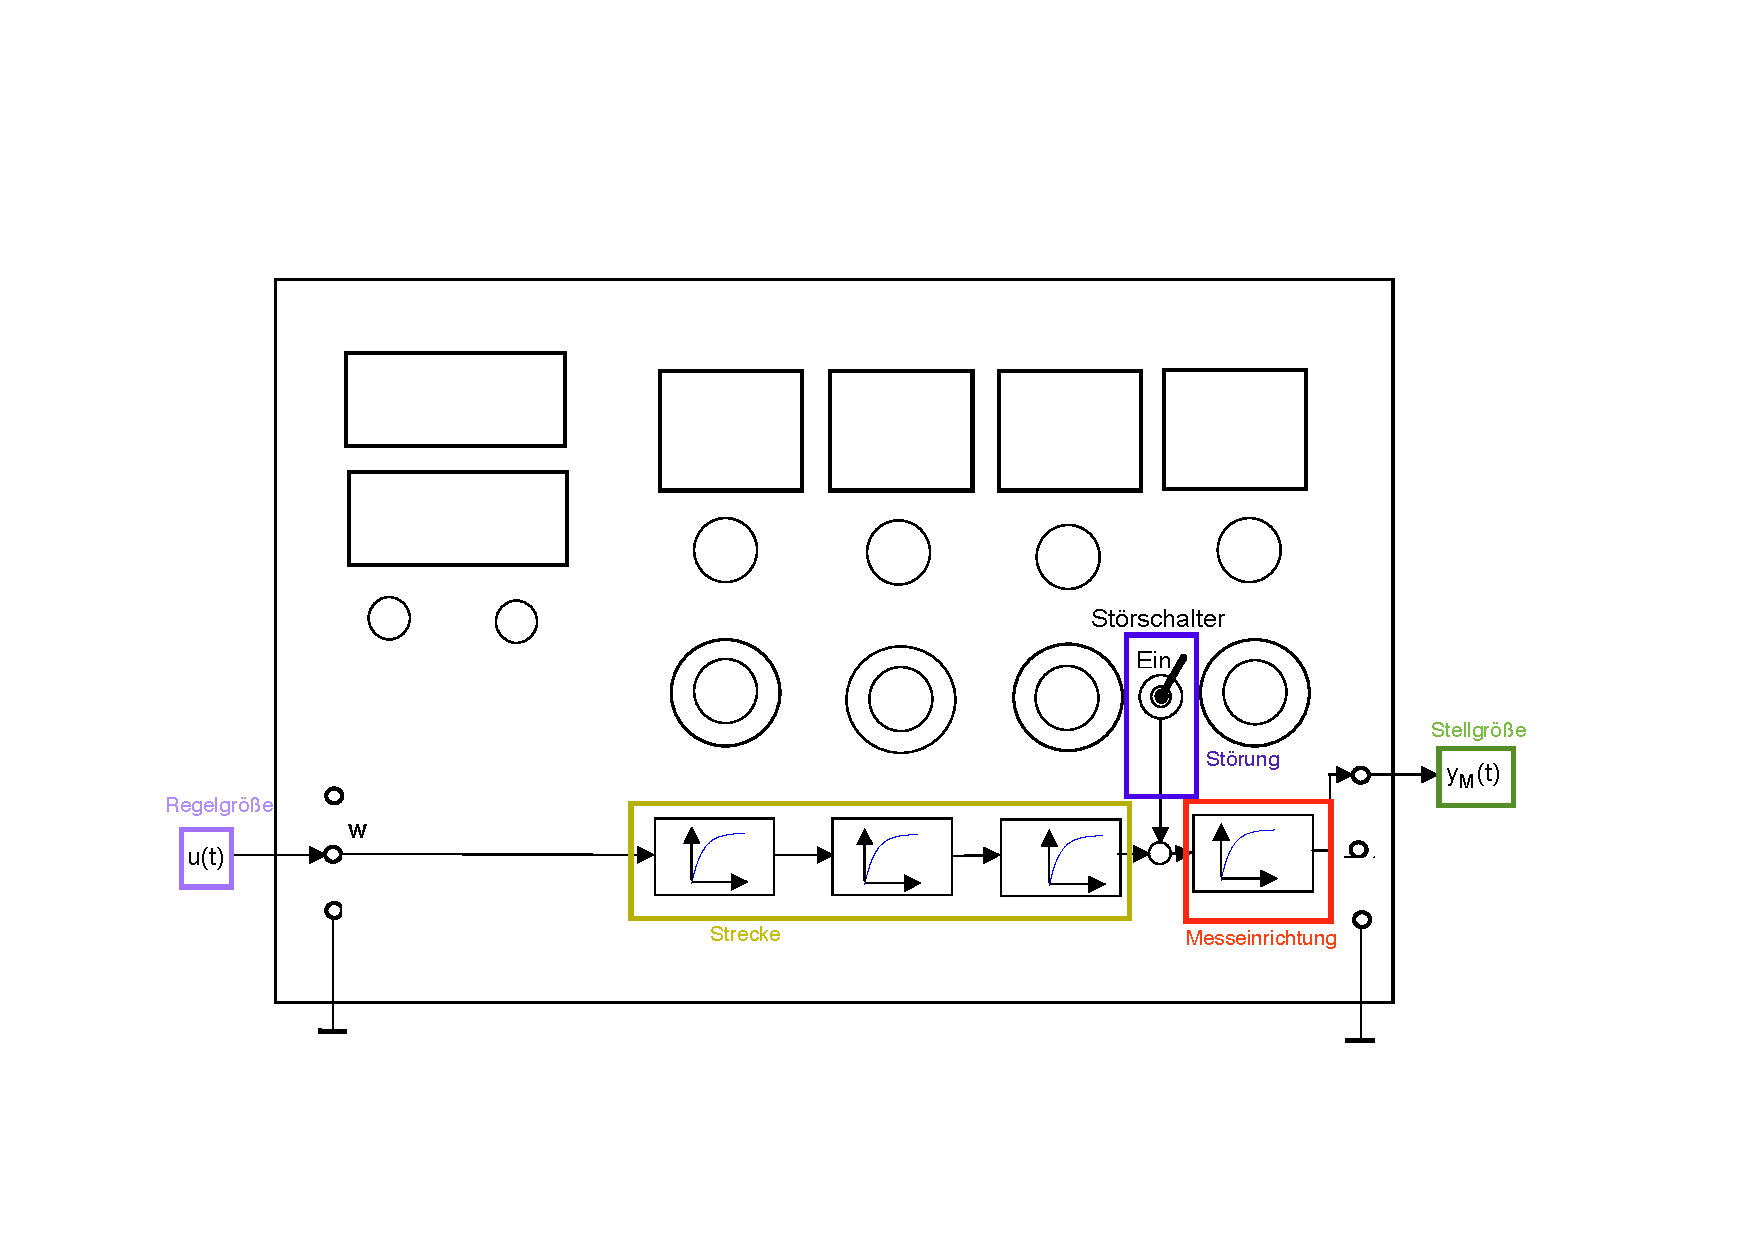
\includegraphics[scale=0.4]{regelkreis.pdf}
		\caption{Elektrische simulierte Druckregelstrecke mit Standard-Regelkreis}
       \label{RegelKreis}
	\end{center} 
\end{figure}

\newpage

Um alle Größen zu bestimmen/messen und der Reger zu entwickeln wird MATLAB/Simulink eingesetzt. Dies geschieht mit das Tool Real-Time-Workshop und eine A/D-D/A Wandlerkarte.


\subsection{Offset}
Um das System mit dem Rechner zu verbinden wird eine Wandlerkarte eingesetzt. Die Wandlerkarte ist im PC eingebaut. Um Fälschungen im Ergebnis zu umgehen muss der Eingang- und Ausgangsoffset gemessen werden. Um diese Werte zu messen wurde das \textit{reinraus2007b.mdl} Simulinkmodell benutzt.\\

Für den Eingangsoffset der Wandlerkarte wurde ein Display für die Ausgabe benutzt. Wichtig ist, dass die Leitungen für die Verbindung von der Wandlerkarte zum System kurzgeschlossen werden. Auf dieser Weise werden zum Beispiel $5V$ angelegt und diese $5V$ werden vom Ergebnis subtrahiert. Unser Eingangsoffset beträgt $0,1292V$.\\

Um den Ausgangsoffset zu ermitteln werden die zwei Leitungen an ein Voltmeter angeschlossen. Dieser sollte bei kein Offset $0$ zeigen. Im unser Fall konnten wir ein Ausgangsoffset von $0,1050V$ ablesen.\\

Diese beide Werte werden bei Simulationen in den Kapiteln \ref{Kapitel5} und \ref{Kapitel7} jeweils  subtrahiert um die Verfälschung von Ergebnisse zu vermeiden.


%%%%%%%%%%%%%%%%%%%%%%%%%%
%% bild einfügen

%\begin{figure}[h]
%	\begin{center}
%		\includegraphics[scale=0.5]{pic.jpg}
%		\caption{bildbeschreibung - titel}
%       \label{für referenzen}
%	\end{center} 
%\end{figure}